%% LyX 1.6.5 created this file.  For more info, see http://www.lyx.org/.
%% Do not edit unless you really know what you are doing.
\documentclass[10pt,twocolumn,english,times]{article}
\usepackage[T1]{fontenc}
\usepackage[latin9]{inputenc}
\pagestyle{empty}
\usepackage{graphicx}

\makeatletter
%%%%%%%%%%%%%%%%%%%%%%%%%%%%%% Textclass specific LaTeX commands.
\newenvironment{lyxcode}
{\par\begin{list}{}{
\setlength{\rightmargin}{\leftmargin}
\setlength{\listparindent}{0pt}% needed for AMS classes
\raggedright
\setlength{\itemsep}{0pt}
\setlength{\parsep}{0pt}
\normalfont\ttfamily}%
 \item[]}
{\end{list}}

%%%%%%%%%%%%%%%%%%%%%%%%%%%%%% User specified LaTeX commands.

%  $Description: Author guidelines and sample document in LaTeX 2.09$ 
%  $Author: ienne $
%  $Date: 1995/09/15 15:20:59 $
%  $Revision: 1.4 $
\usepackage{latex8}\usepackage{times}

%\documentstyle[times,art10,twocolumn,latex8]{article}
%------------------------------------------------------------------------- 
% take the % away on next line to produce the final camera-ready version 


%------------------------------------------------------------------------- 

\makeatother

\usepackage{babel}

\begin{document}

\title{Really Awesome Distributed Internet Calendar (RADICAL)}


\author{Lalith Suresh P.\\
DEI\\
Instituto Superior Tecnico\\
Lisbon, Portugal\\
suresh.lalith@gmail.com\\
\and Marcus Ljungblad\\
DEI\\
Insituto Superior Tecnico\\
Lisbon, Portugal\\
marcus@ljungblad.nu\and Bruno Pereira\\
DEI\\
Insituto Superior Tecnico\\
Lisbon, Portugal\\
brunopereir4@gmail.com}

\maketitle
\thispagestyle{empty}
\begin{abstract}
Shared calendar systems like Google Calendar are known to be an effective
way for people to schedule and coordinate events. In this project,
we design and implement PADICal, a peer-to-peer based distributed
calendar system. PADICal allows clients to make event reservations
amongst themselves in an almost decentralised manner with minimal
assistance from a central server.
\end{abstract}

\section{Introduction}

The aim of this project is to design, implement and evaluate a shared
calendar system which has the following components:
\begin{itemize}
\item Multiple clients, each with their own calendars, who may contact one
another to schedule events together.
\item A centralised server which holds usernames and provides clients a
sequence number service.
\end{itemize}
The rest of the paper is organised as follows: Section \ref{sec:systemarch}
describes the architecture of the different components of the system.


\section{System Architecture\label{sec:systemarch}}

Since there is a Client and Server entity for this system, we describe
the architecture of each separetely. One of the main design goals
is to allow easy testability and debugging facilities within the system
in order to ease development. To a certain degree, we hope to achieve
this through classic 'printf' style debugging. Every class in PADICal
inherits from a class \texttt{PadiCalObject}, which has two virtual
methods named \texttt{Debug() }and \texttt{UnitTests()}. The former
performs pretty printing of internal state of an object, and follows
the flow of logic through the stack whereas the latter is written
during the development phase to ensure methods do not misbehave when
changes are introduced later. All sub classes have to implement these
methods depending on the kind of methods and state information they
may hold. The \texttt{Debug()} method of different objects comprising
of a client or server can be enabled via a configuration file or through
some interfaces we can provide to the UI of the client.

The client and the server architecture has been logically decomposed
into 3 layers each. From top to down, they are as follows: the interface
layer, the services layer, and the communications layer. In the sections
below, we first describe the client, the server, and the components
of each of the 3 layers that they comprise of.


\subsection{Client}

%
\begin{figure*}
\begin{centering}
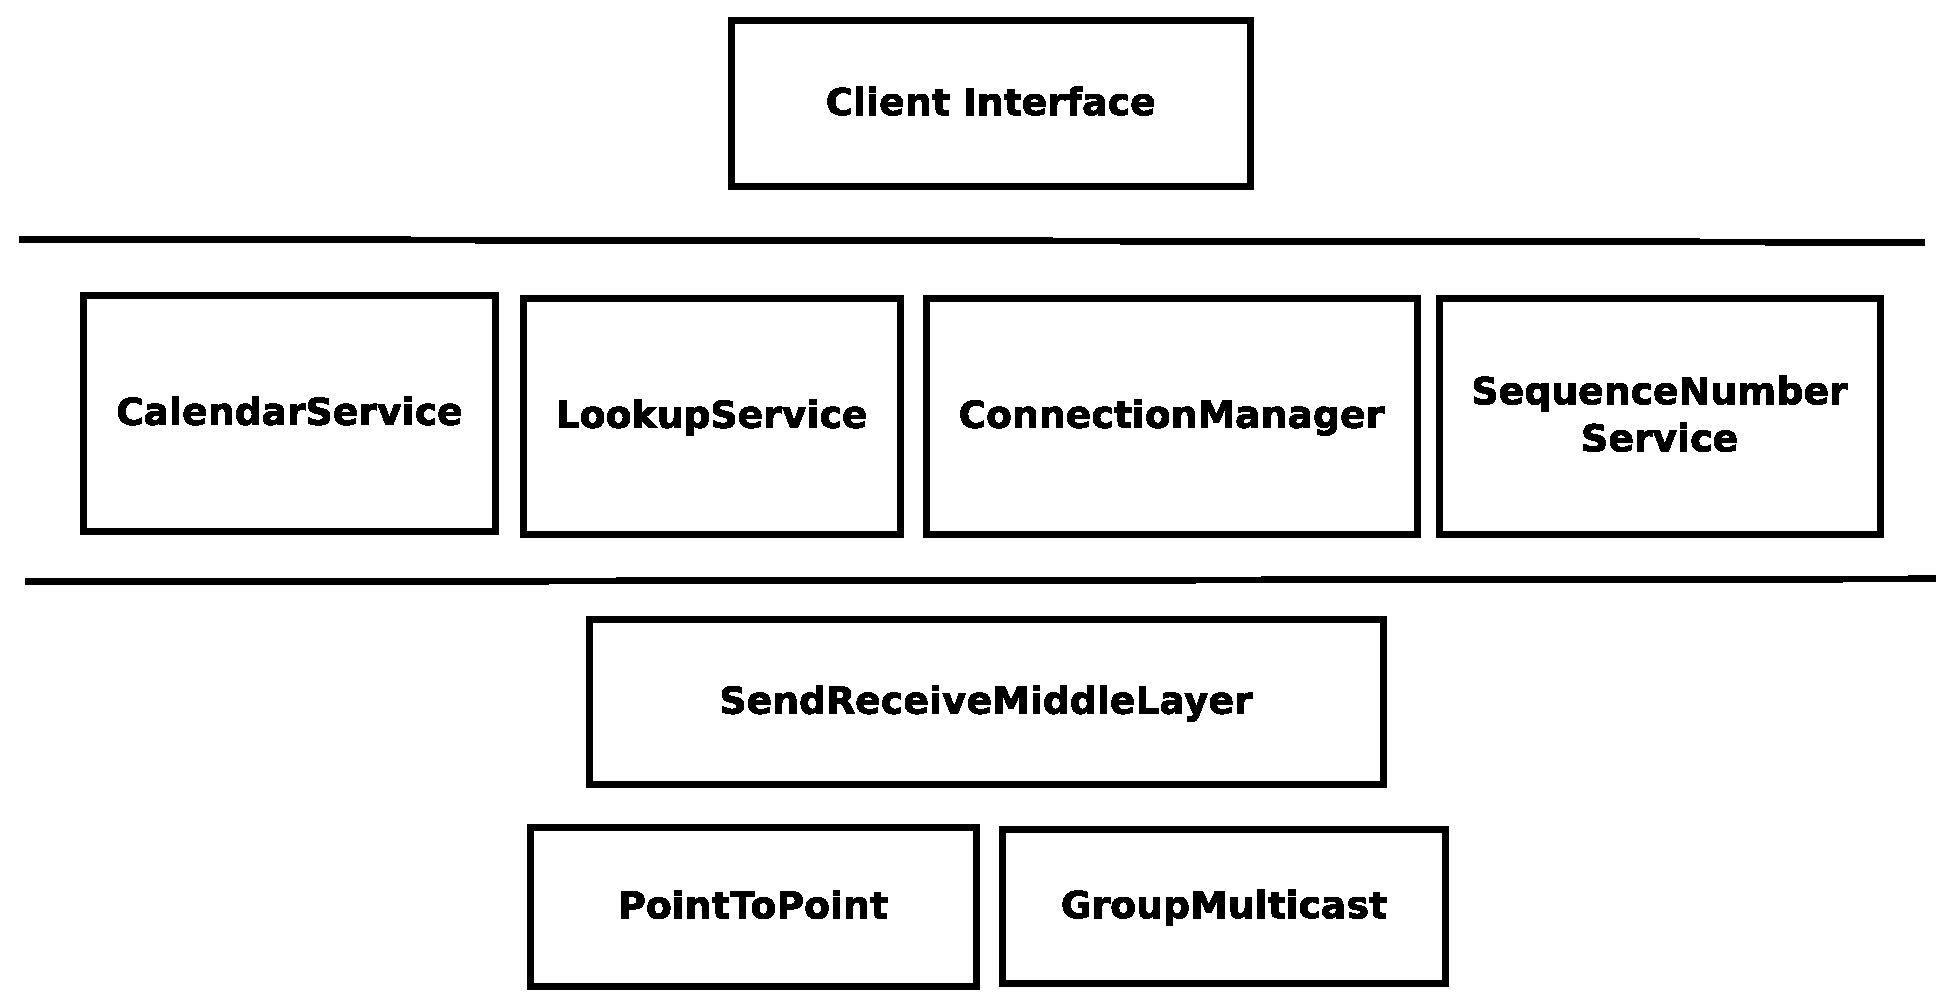
\includegraphics[scale=0.25]{client}
\par\end{centering}

\caption{Client Architecture. A 3 layer approach is used, with the following
stack: An interface layer (\texttt{Client Interface}), a service layer
(\texttt{CalendarService, LookupService, ConnectionManager, SequenceNumberService})
and a communication layer (\texttt{SendReceiveMiddleLayer, PointToPoint,
GroupMulticast}).\label{fig:clientarch}}

\end{figure*}


The client architecture is described in Figure. \ref {fig:clientarch}.
The working of the client has been decomposed into three layers, each
of which holds the appropriate working components. This is described
as follows:


\subsubsection{Interface Layer}

The client's interface layer comprises of the following:
\begin{itemize}
\item \texttt{Client Interface}: The instantiation of this class handles
user inputs. The user can reserve events on the calendar, view the
calendar and connect/disconnect to the server.
\end{itemize}

\subsubsection{Services Layer}
\begin{itemize}
\item \texttt{CalendarService}: This is the abstraction for the calendar
itself. The event reservation and commit protocols are implemented
within this class.
\item \texttt{LookupService}: The Client performs lookups over the usernames
of other participants using this service. The (IP,Port) tuples returned
for each username are used to describe connections and remote object
invocations for every other component in the system.
\item \texttt{ConnectionManager}: This component handles user login/sign-outs.
\item \texttt{SequenceNumberService}: This service provides a unique sequence
number from the centralised servers.
\end{itemize}

\subsubsection{Communications Layer}
\begin{itemize}
\item \texttt{SendReceiveMiddleLayer}: To abstract the underlying communication
process from the services, we use the \texttt{SendReceiveMiddleLayer}.
If there are multiple recipients to send a message to, this layer
uses the \texttt{GroupMulticast }abstraction, else, uses the \texttt{PointToPoint
}abstraction. It also acts as a demultiplexer (on the same lines as
Linux's \texttt{{}``}layer 4 demux\texttt{''}), to find the appropriate
service layer recipient for a particular message.
\item \texttt{GroupMulticast}: This abstraction uses the \texttt{PointToPoint
}abstraction to deliver messages to a group of participants.
\item \texttt{PointToPoint}: This abstraction uses a remote invocation to
send a message to a recipient.
\end{itemize}

\subsection{Server}

The Radical server consists of one master and three replicas. Each
replica is strongly consistent with the master and updated on each
write. In this section we describe the architecture of the servers,
including the replicas, its leader election process, and its interfaces.
The services provided by the server are: a user to (IP, Port) lookup
table and sequence numbering. A server instance may be in one of two
states: master or replica. As a master, the instance is the primary,
and only, responsible for serving clients with data. We assume that
at most one instance may fail at any time during normal execution,
including the master. If the master instance becomes unavailable,
a new master is automatically elected among the three replicas. 
\begin{lyxcode}
%
\begin{figure*}[t]
\begin{centering}
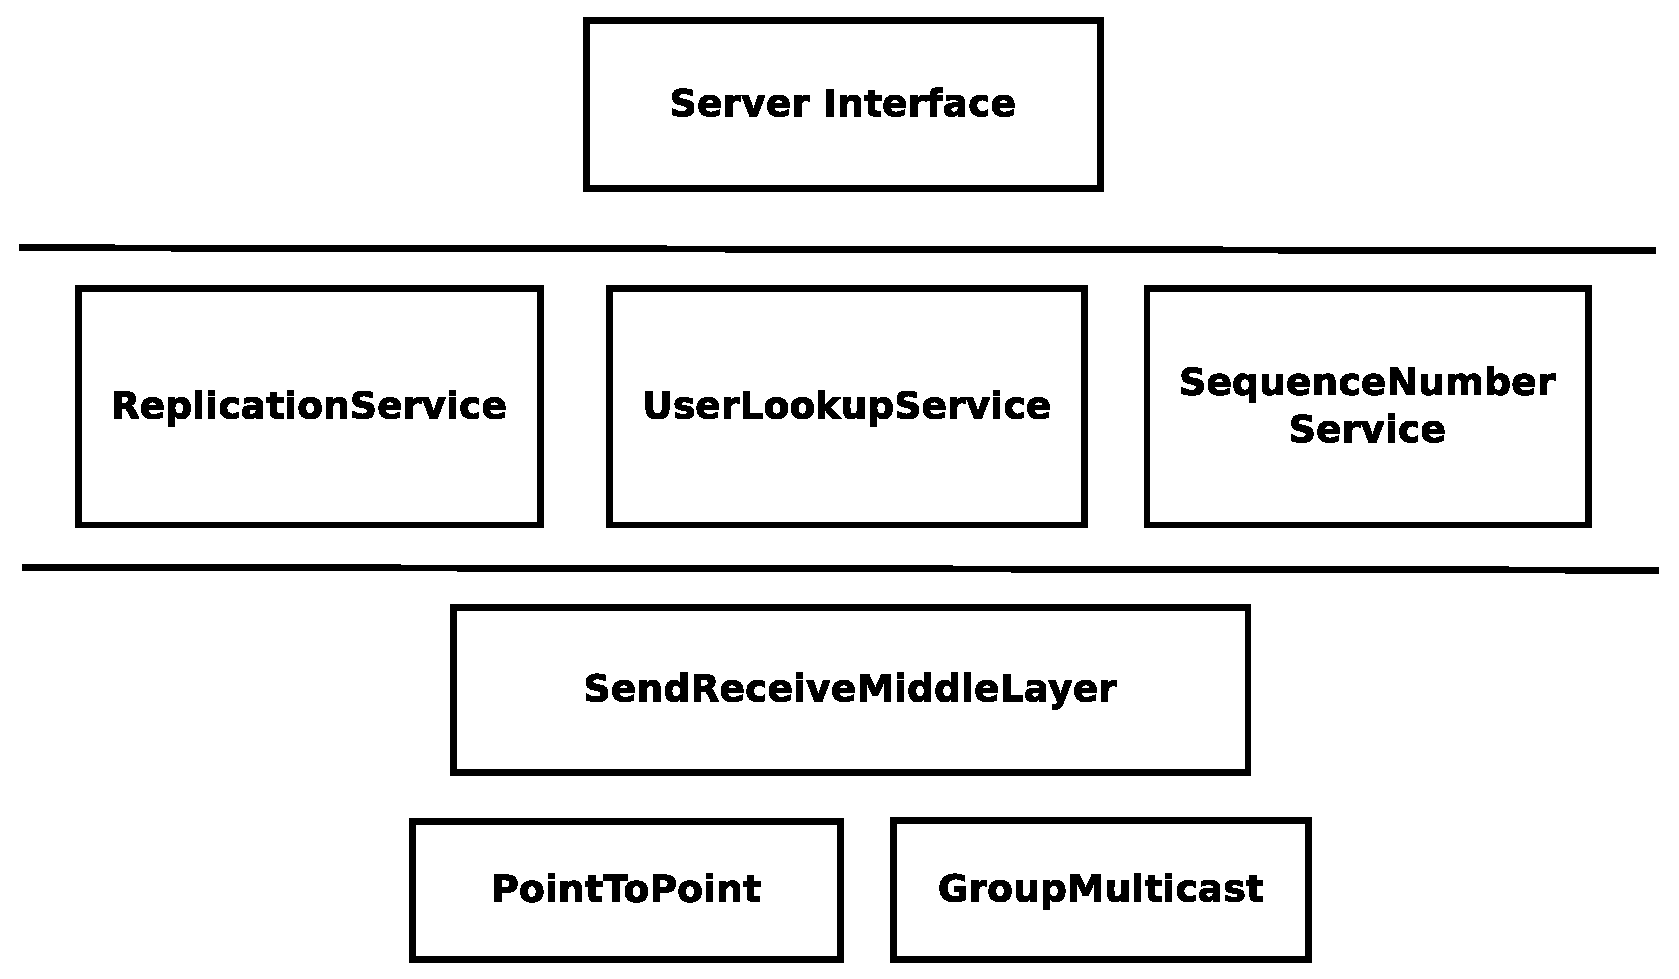
\includegraphics[scale=0.25]{server}
\par\end{centering}

\caption{Server Architecture. A 3 layer approach is used, with the following
stack: An interface layer (\texttt{ServerInterface}), a service layer
(\texttt{ReplicationService, UserLookupService, SequenceNumberService})
and a communication layer (\texttt{SendReceiveMiddleLayer, PointToPoint,
GroupMulticast}).\label{fig:serverarch}}

\end{figure*}

\end{lyxcode}

\subsubsection{Interface Layer}

The client's interface layer comprises of the following:
\begin{itemize}
\item \texttt{Server Interface}: The instantiation of this class handles
user inputs. The user can view server state, the currently active
replica, and the currently logged on users.
\end{itemize}

\subsubsection{Services Layer}
\begin{itemize}
\item \texttt{ReplicationService}: This is the abstraction for the strongly
consistent replication service.
\item \texttt{UserLookupService}: This service handles both connect/disconnects
from the clients, and also provides the required username to (IP,
Port) lookup service for them.
\item \texttt{SequenceNumberService}: This service provides a unique sequence
number to the clients.
\end{itemize}

\subsubsection{Communications Layer}
\begin{itemize}
\item The components of the server communications layer remains the same
as that of the client.
\end{itemize}

\section{Algorithms}


\subsection{Client Side: Reservation/Commit Protocol}

The reservation protocol follows the steps as outlined in the project
description. Once a client is in the tentatively booked state for
a particular event slot, it executes the commit protocol.

We have opted to use a modified 3-phase commit algorithm (ref) which
works as follows:
\begin{itemize}
\item Coordinator side (initiator of the event reservation):

\begin{enumerate}
\item The coordinator receives a transaction request. If there is a failure
at this point, the coordinator aborts the transaction (i.e. upon recovery,
it will consider the transaction aborted). Otherwise, the coordinator
sends a canCommit? message to the cohorts and moves to the waiting
state.
\item If there is a failure, timeout, or if the coordinator receives a No
message in the waiting state, the coordinator aborts the transaction
and sends an abort message to all cohorts. Otherwise the coordinator
will receive Yes messages from all cohorts within the time window,
so it sends preCommit messages to all cohorts and moves to the prepared
state.
\item If the coordinator succeeds in the prepared state, it will move to
the commit state. However if the coordinator times out while waiting
for an acknowledgement from a cohort, it will abort the transaction.
In the case where all acknowledgements are received, the coordinator
moves to the commit state as well, and sends a doCommit message to
all participants indicating that they can commit right away (and not
wait for their abort/commit timeouts).
\end{enumerate}
\item Cohort side (other participants in reservation):

\begin{enumerate}
\item The cohort receives a canCommit? message from the coordinator. If
the cohort agrees it sends a Yes message to the coordinator and moves
to the prepared state. Otherwise it sends a No message and aborts.
If there is a failure, it moves to the abort state.
\item In the prepared state, if the cohort receives an abort message from
the coordinator, fails, or times out waiting for a commit, it aborts.
If the cohort receives a preCommit message, it sends an ACK message
to the coordinator. It then initiates a commit timeout and verify
timeout. The verify timeout is shorter than the commit timeout and
is higher than the minimum time required for the ACK message to reach
the coordinator. If the client receives a 'doCommit' message before
either timeout, then it commits.
\item Since every participant is aware of the list of participants in the
reservation, it is trivial to arrange all the participants (including
the coordinator) in a circle (since the coordinator sends all participants
the same list). At the point of verify timeout, the nodes ping their
left and right neighbours in the ring. If a participant does not receive
a pong for its ping, then it detects that a partition could have occured
and does not commit, and informs the coordinator and its other neighbour
that to abort. We assume symmetrical links in the system, that is,
if A cannot ping B, then B cannot ping A. The message can then be
disseminated in broadcast or tree patterns in order to ensure a quick
abort by all nodes. If the verify phase succeeds, nodes can commit
once the commit timeout occurs.
\end{enumerate}
\end{itemize}
The cohort's execution of verifying whether its left and right neighbours
are alive before committing ensures that a network partition has not
occurred and all nodes are moving into the same state. The verify
timer being shorter than the commit timer protects against the scenario
where some nodes proceed with a commit, while the others abort. Any
node that fails in between the above procedure executes an orderly
leave and can thus abort the process, removing the need for a leader-election
and quorum based solution in case of network partitions like the Enhanced
3PC offers \cite{idit}.

The possibility of a deadlock exists in the phase where two clients
are involved in at least two common event reservations. It can happen
that two clients which are in the tentatively booked phase for the
same two events, initiate their commit protocols, but receive the
pre-commit messages in different order. This can be either handled
by using a wait-queue, or by having each client abort the later commit
sequence. The latter would lead to both reservation processes aborting.
This is safe, but we plan to optimise this part such that one of them
will proceed with a commit.


\subsection{Server Side: Leader Election and Replication}


\subsubsection{Leader Election}

All instances of a server knows about all other server instances.
Each instance has a unique id. Since the number of servers never exceeds
four, each server regularly emits a heartbeat to let the other servers
know it is alive. It is assumed that at most one server may fail at
any time. During the bootstrap of a server, each instance will select
the server with the highest ID to be the leader. Our leader election
process is based on the Bullying algorithm proposed by \cite{GarciaMolina}.
In case of a server failure, when any other instance suspects that
a server is unavailable, it will send a proposal to all other servers
that X is unavailable. If all others agree, the server with the next
highest ID is elected the new leader. The leader is selected in a
round-robin fashion. To handle network partitions, a server may only
become a leader if it is part of the cluster with a majority of the
servers. In case each cluster is of equal size, the cluster with the
current (or previous) leader will remain/elect the leader. Clients
trying to contact the minority cluster will not get any replies, and
according to the round-robin selection scheme, eventually pick a server
from the majority cluster. 


\subsubsection{Replication}

In the interface above, three of the interfaces are considered writes.
Since we want to maintain a strong consis- tency among the replicas,
the master instance will propagate a write to all replicas before
replying to the client. The propagation is assumed to be synchronous
and utilises the broadcast component of the communication layer described
earlier. Since performance is not one of the main non-functional requirements
of this system, a server which receives a request will block until
it receives an acknowl- edgement from all correct replicas. A replica
is considered correct as long as a heartbeat has been received within
the given timeframe. It is worth adding here that an optimisation
to this algorithm is to consider only acks from a subset of the replicas.
In the event of such optimization it is neces- sary to establish an
auxilliary mechanism to ensure that all replicas are in a consistent
state. In case a replica, i.e an instance which is not the leader,
gets an unexpected request from a client it will query the leader
for the data, and retransmit the response to the client. Before propagating
write requests to replicas, the leader maintains a log of all write
records. When a server fails, and after a new leader is elected, the
server instances will synchronize to ensure that the user lookup table
and sequence number is aligned. Each write to the user lookup table
is associated with a logical timestamp, such that ordering can be
guaranteed. TBD: how to manage network partition for replication propagation. 


\subsection{Possible Optimisations}

Some possible optimisations that we will work on once we get a basic
version of the code include:
\begin{itemize}
\item Minimising username lookups from the client side by using a cache
(in the same lines as a DNS cache).
\item In the scheme for committing a reservation, it is possible that two
clients can be part of two reservation sequences, and each of them
can abort each other's sequences. This is a safety measure, but it
is possible to use a tie-breaking system at the tentatively booked
phase.
\end{itemize}
\bibliographystyle{latex8}
\bibliography{latex8}

\end{document}
